\documentclass[
  bibliography=totoc,     % Literatur im Inhaltsverzeichnis
  captions=tableheading,  % Tabellenüberschriften
  titlepage=firstiscover, % Titelseite ist Deckblatt
]{scrartcl}

% Paket float verbessern
\usepackage{scrhack}

% Warnung, falls nochmal kompiliert werden muss
\usepackage[aux]{rerunfilecheck}

% unverzichtbare Mathe-Befehle
\usepackage{amsmath}
% viele Mathe-Symbole
\usepackage{amssymb}
% Erweiterungen für amsmath
\usepackage{mathtools}

% Fonteinstellungen
\usepackage{fontspec}
% Latin Modern Fonts werden automatisch geladen
% Alternativ zum Beispiel:
%\setromanfont{Libertinus Serif}
%\setsansfont{Libertinus Sans}
%\setmonofont{Libertinus Mono}

% Wenn man andere Schriftarten gesetzt hat,
% sollte man das Seiten-Layout neu berechnen lassen
\recalctypearea{}

% deutsche Spracheinstellungen
\usepackage[ngerman]{babel}

\usepackage[table]{xcolor}

\usepackage[
  math-style=ISO,    % ┐
  bold-style=ISO,    % │
  sans-style=italic, % │ ISO-Standard folgen
  nabla=upright,     % │
  partial=upright,   % ┘
  warnings-off={           % ┐
    mathtools-colon,       % │ unnötige Warnungen ausschalten
    mathtools-overbracket, % │
  },                       % ┘
]{unicode-math}

% traditionelle Fonts für Mathematik
\setmathfont{Latin Modern Math}
% Alternativ zum Beispiel:
%\setmathfont{Libertinus Math}

\setmathfont{XITS Math}[range={scr, bfscr}]
\setmathfont{XITS Math}[range={cal, bfcal}, StylisticSet=1]

% Zahlen und Einheiten
\usepackage[
  locale=DE,                   % deutsche Einstellungen
  separate-uncertainty=true,   % immer Unsicherheit mit \pm
  per-mode=symbol-or-fraction, % / in inline math, fraction in display math
]{siunitx}

% chemische Formeln
\usepackage[
  version=4,
  math-greek=default, % ┐ mit unicode-math zusammenarbeiten
  text-greek=default, % ┘
]{mhchem}

% richtige Anführungszeichen
\usepackage[autostyle]{csquotes}

% schöne Brüche im Text
\usepackage{xfrac}

% Standardplatzierung für Floats einstellen
\usepackage{float}
\floatplacement{figure}{htbp}
\floatplacement{table}{htbp}

% Floats innerhalb einer Section halten
\usepackage[
  section, % Floats innerhalb der Section halten
  below,   % unterhalb der Section aber auf der selben Seite ist ok
]{placeins}

% Seite drehen für breite Tabellen: landscape Umgebung
\usepackage{pdflscape}

% Captions schöner machen.
\usepackage[
  labelfont=bf,        % Tabelle x: Abbildung y: ist jetzt fett
  font=small,          % Schrift etwas kleiner als Dokument
  width=0.9\textwidth, % maximale Breite einer Caption schmaler
]{caption}
% subfigure, subtable, subref
\usepackage{subcaption}

% Grafiken können eingebunden werden
\usepackage{graphicx}

% schöne Tabellen
\usepackage{booktabs}

% Verbesserungen am Schriftbild
\usepackage{microtype}

% Literaturverzeichnis
\usepackage[
  backend=biber,
]{biblatex}
% Quellendatenbank
\addbibresource{lit.bib}
%\addbibresource{programme.bib}
%\bibliographystyle{plain}
%\bibliography{lit.bib}

% Hyperlinks im Dokument
\usepackage[
  german,
  unicode,        % Unicode in PDF-Attributen erlauben
  pdfusetitle,    % Titel, Autoren und Datum als PDF-Attribute
  pdfcreator={},  % ┐ PDF-Attribute säubern
  pdfproducer={}, % ┘
]{hyperref}
% erweiterte Bookmarks im PDF
\usepackage{bookmark}

% Trennung von Wörtern mit Strichen
\usepackage[shortcuts]{extdash}

\author{%
  AUTOR A\\%
  \href{mailto:authorA@udo.edu}{authorA@udo.edu}%
  \and%
  AUTOR B\\%
  \href{mailto:authorB@udo.edu}{authorB@udo.edu}%
}
\publishers{TU Dortmund – Fakultät Physik}


\subject{V101}
\title{Das Trägheitsmoment}
\author{Umut Aydinli \\
 \href{mailto:umutaydinli27@gmail.com}{umutaydinli27@gmail.com}
 \and Muhammed-Sinan Demir \\
 \href{mailto:sinan.demir@tu-dortmund.de}{sinan.demir@tu-dortmund.de}
 }
\date{
  Durchführung: 26.11.2021
  \hspace{3em}
  Abgabe: 03.12.2021
}


\begin{document}

\maketitle
\tableofcontents
\newpage

\section{Zielsetzung} 

\begin{flushleft}
    In dem Versuch V602 geht es um die Bestimmung des Emissionsspektrums einer Kupferröntgenröhre, das Absorptionsspektrum verschiedener Stoffe und die Überprüfung der Bragg Bedingung. 
\end{flushleft}



\section{Theorie}


\begin{flushleft}
    Licht besteht aus elektromagnetischen Wellen und ist somit durch die Maxwell Gleichungen beschreibbar.
    Licht, welches im sichtbaren Bereich liegt, hat eine Wellenlänge zwischen $380\unit{\nano\meter}$ und $780\unit{\nano\meter}$.
    Das Ultraviolette Spektrum liegt unter den $380\unit{\nano\meter}$ bzw. zwischen $100\unit{\nano\meter}$ und $380\unit{\nano\meter}$, wobei das Infrarotspektrum über den $780\unit{\nano\meter}$ liegt, genauer gesagt zwischen $780\unit{\nano\meter}$ und $1\unit{\milli\meter}$
\end{flushleft}

\subsection{Strahlenoptik}

\begin{align}
    \intertext{Die Wellennormale beschreibt in der Strahlenoptik die Ausbreitung der Welle.
    Dabei ist die Ausbreitungsgeschwindigkeit unterschiedlich groß, welches von dem Material abhängt.
    Beim Auftreffen eines Lichtstrahles auf die Grenzfläche eines Mediums wird der Lichtstrahl gebrochen.
    Dabei entstehen zwei Ausbreitungsgeschwindigkeiten, $\text{v}_{1}$ und $\text{v}_{2}$, die durch die beiden Brechungsindizes der Medien, $\text{n}_{1}$ und $\text{n}_{2}$, sowie durch den Einfallswinkel $\alpha$ und Brechungswinkel $\beta$ beschrieben werden können  }
    \frac{\sin(\alpha)}{\sin(\beta)} = \frac{\text{v}_{1}}{\text{v}_{2}} = \frac{\text{n}_{2}}{\text{n}_{1}}\,. \label{1}
    \intertext{Luft ist ebenfalls ein Medium, dessen Ausbreitungsgeschwindigkeit bei $ \text{v}_{1} = 2,9979 \cdot 10^{8} \frac{\unit{\meter}}{\unit{\second}} $ liegt und einen Brechungsindex von $\text{n}_{1} = 1,000292$ besitzt.
    Das Medium,in welchen die Ausbreitungsgeschwindigkeit des Lichts größer ist als in dem anderen Medium, gilt als optisch dichteres Medium.
    Dadurch gilt, dass bei geringerer Ausbreitungsgeschwindigkeit von einem optisch dünneren Medium gesprochen wird.  }
\end{align}

\subsection{Reflexion} 

\begin{align}
    \intertext{Das Reflexionsgesetz besagt, dass wenn ein Lichtstrahl auf eine Grenzfläche auftrifft und reflektiert wird, ist der Einfallswinkel gleich dem Ausfallswinkel }
    \alpha_{1} = \alpha_{2}\,. \label{2}
\end{align}

\begin{figure}[H]
    \centering
    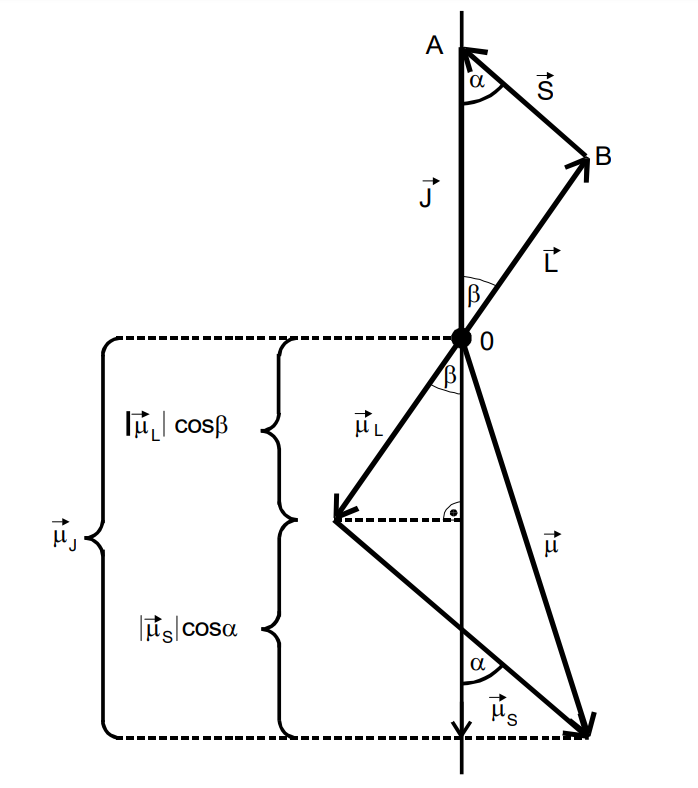
\includegraphics[height=40mm]{bilder/Ab1.png}
    \caption{Das reflektieren eines Lichtstrahles \cite{a1}.\label{Abbildung1} }
\end{figure}


\subsection{Brechung} 

\begin{align}
    \intertext{Brechung des Lichtes wird mit dem Snellius Gesetz erklärt, welches besagt, dass beim Auftreffen eines Lichtstrahl auf ein anderes Medium mit einem Brechungsindex n, dieser gebrochen wird.
    Dadurch wird der Ausfallswinkel als $\beta$ beschrieben}
    \text{n}_{1} \sin(\alpha) = \text{n}_{2} \sin(\beta)\,.\label{3}
\end{align}

\begin{figure}[H]
    \centering
    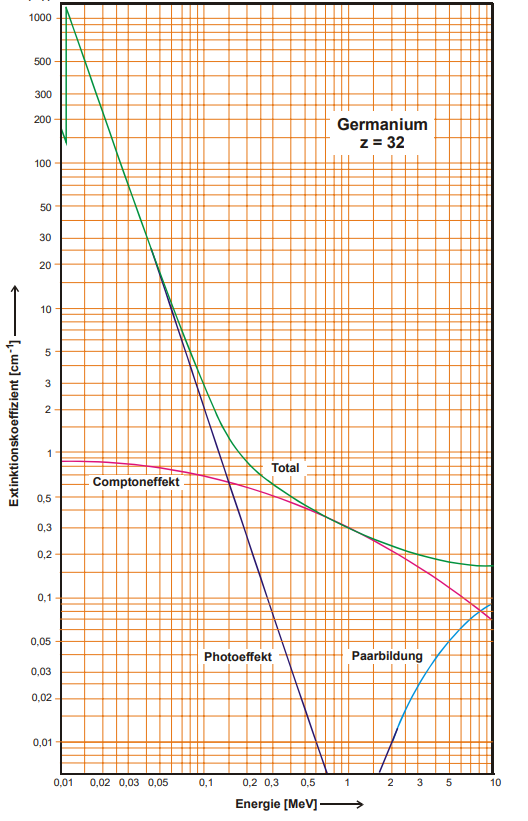
\includegraphics[height=45mm]{bilder/Ab2.png}
    \caption{Das brechen eines Lichtstrahles \cite{a1}. \label{Abbildung2} }
\end{figure}

\subsection{Reflexion und Transmission}

\begin{align}
    \intertext{Oft wird Licht nicht vollständig reflektiert, wenn es auf die Grenzfläche eines Mediums trifft.
    Der Teil des Lichtstrahles, der nicht reflektiert wird, wird transmittiert bzw. gebrochen.
    Dabei gilt das der Teil der reflektiert wird und der Teil der gebrochen wird, zusammen 1 ergibt}
    \text{R} + \text{T} = 1\,. \notag
\end{align}

\begin{figure}[H]
    \centering
    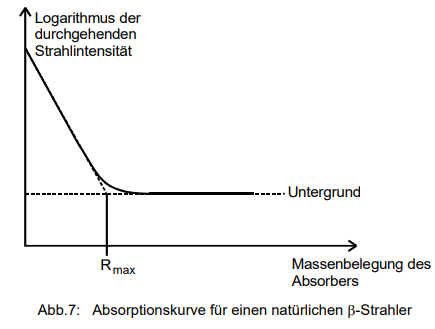
\includegraphics[height=45mm]{bilder/Ab3.png}
    \caption{Das reflektieren und brechen eines Lichtstrahles \cite{a1}. \label{Abbildung3} }
\end{figure}

\subsection{Wellenoptik}

\begin{flushleft}
    Beim Auftreffen des Lichtes auf ein Objekt, welches im Verhältnis zur Wellenlänge klein ist, breitet sich dieses auch im Schattenraum aus, da die geometrische Optik dafür nicht mehr ausreicht.
    Dabei sind Frequenz f, Wellenlänge $\lambda$ und Ausbreitungsgeschwindigkeit v, charakteristische Merkmale einer Welle, dessen Wellenzüge nicht länger als $10^{-8}\,\unit{\second}$ dauern.
    Durch eine Superpostion der Wellen können dennoch Interferenzbilder entstehen, wobei unter konstruktiver und destruktiver Interferenz unterschieden wird. 
    Beträgt der Gangunterschied bei gleicher Intensität $\lambda/2$, führt dies zu einer vollständigen Auslöschung der Welle.
\end{flushleft}

\subsection{Beugung am Gitter}

\begin{align}
    \intertext{Liegt bei der Ausbreiten der Lichtwelle ein Hindernis auf dem Weg, welches im Vergleich zur Wellenlänge klein ist, so kann es zu einer Beugung führen.
    Das Huygensche Prinzip beschreibt diese Ausbreitung und besagt, dass jeder Punkt auf einer Wellenfront eine neue Elementarwelle, welche die gleiche Frequenz hat, erzeugt.
    Befindet sich nun ein Spalt im Abstand L mit einem Schirm dahinter, wird ein Interferenzmuster beobachtbar. 
    Die dabei entstehenden Interferenzmaxima ergeben sich durch   }
    \text{a}\,\,\sin(\alpha) = \text{k}\,\lambda \,, \label{4}
    \intertext{wobei a die Spaltbreite, k das k-te Intensitätsminimum und $\lambda$ die Wellenlänge darstellt.
    Diese Intensitätsminima befindet sich in einem Winkel von $\alpha$ relativ zur geradlinigen Ausbreitungsrichtung.
    Dieses Prinzip lässt sich auf ein Strichgitter mit n-Einfachspalten gleicher Breite, mit der Gitterkonstante d, übernehmen.
    Dadurch ergibt sich für die Interferenzmaxima k-ter Ordnung die Beziehung }
    \text{d}\,\,\sin(\alpha) = \text{k}\,\lambda\,. \label{5}
\end{align}
\section{Aufgaben}

\begin{flushleft}
    Zunächst wird die Winkelgröße $ D $ und das dazugehörige Eigenträgheitsmoment ${l}_{\text{D}}$ durch Anwendung des Satzes von Steiner, bestimmt.
    Danach soll das Trägheitsmoment $ l $ von den zwei Körpern bestimmen und mit den theoretisch berechneten Werten vergleichen. 
    Als letztes soll das Trägheitsmoment einer Modellpuppe bestimmt werden, welche in zwei verschiedene Haltungen eingestellt wird.
    Die ermittelten Werte sollen dann verglichen werden mit der dazugehörigen Modellrechnung. 
\end{flushleft}
\section{Vorbereitungsaufgaben}

\begin{align}
    \intertext{Die Vorbereitungsaufgabe für diesen Versuch besteht aus dem Berechnen des Drehmoments $ M $.
    An einer Stange wirkt Senkrecht eine Kraft von $ F = 0.1 \,\unit{\newton}$, in einem Winkel von $ \alpha_{1} = 90 \unit{\degree} $. 
    Ebenso soll man $ \alpha_{2} = 45 \unit{\degree} $
    Die Werte sollen in einem Abstandsbereich von 5 bis 25\,cm bestimmt werden.
    Dies soll für 10 verschiedene Abstände berechnet werden. Hierfür wird die Formel}
    M = F \cdot r \cdot \sin{\alpha} \notag
    \intertext{benötigt.}
    \to \quad M_{r1} = 0.1\unit{\newton} \cdot r \cdot \sin{(45 \unit{\degree})} \\
    \to \quad M_{r2} = 0.1\unit{\newton} \cdot r \cdot \sin{(90 \unit{\degree})} 
\end{align}

\begin{align*}
\intertext{die verschiedenen Abstände eingesetzt führen zu den Ergebnissen }
    M_{r1=5}  = 0,353\, \unit{\newton}, \, \, \, \, M_{r2=5}   =  0,5\, \unit{\newton}\\
    M_{r1=7}  = 0,495\, \unit{\newton}, \, \, \, \, M_{r2=7}   =  0,7\, \unit{\newton}\\
    M_{r1=9}  = 0,636\, \unit{\newton}, \, \, \, \, M_{r2=9}  ,=  0,9\, \unit{\newton}\\
    M_{r1=11} = 0,779\, \unit{\newton}, \, \, \, \, M_{r2=11}  =  1,1\, \unit{\newton}\\
    M_{r1=13} = 0,919\, \unit{\newton}, \, \, \, \, M_{r2=13}  =  1,3\, \unit{\newton}\\
    M_{r1=15} = 1,060\, \unit{\newton}, \, \, \, \, M_{r2=15}  =  1,5\, \unit{\newton}\\
    M_{r1=17} = 1,202\, \unit{\newton}, \, \, \, \, M_{r2=17}  =  1,7\, \unit{\newton}\\        
    M_{r1=19} = 1,343\, \unit{\newton}, \, \, \, \, M_{r2=19}  =  1,9\, \unit{\newton}\\
    M_{r1=21} = 1,484\, \unit{\newton}, \, \, \, \, M_{r2=21}  =  2,1\, \unit{\newton}\\
    M_{r1=23} = 1,626\, \unit{\newton}, \, \, \, \, M_{r2=23}  =  2,3\, \unit{\newton}\\
    M_{r1=25} = 1,767\, \unit{\newton}. \, \, \, \, M_{r2=25}  =  2,5\, \unit{\newton}\\
\end{align*}





\newpage
\section{Versuchsaufbau}

\begin{flushleft}
    Der Versuch besteht aus den Einzelteilen: \\

    \vspace{0.3cm}

    Oszilloskop, Frequenzgenerator, RLC-Schaltung in Abbildung \ref{Abbildung4} zu sehen, Kabel, Kabel mit Tastkopf.
    
    \vspace{0.3cm}

    Der Frequenzgenerator wird über ein Kabel mit der RLC Schaltung (dem Gerät 1) verbunden.
    Die Schaltung besteht aus einer Reihenschaltung bestehend aus Spule mit Induktivität \textbf{L} und Kondensator mit Kapazität \textbf{C}. 
    In der Serienschaltung sind parallel Widerstände geschaltet. 
    Zwei davon sind fest Widerstände \textbf{R} und einer ein variabler Widerstand $\symup{\text{R}_\text{variabel}}$.

    \vspace{0.5cm}

    Der variable Widerstand wird über einen Regler am Gerät eingestellt und umfasst einen Widerstand von bis zu $10\,\unit{\kilo\ohm}$.
    Die Schaltung ist über ein Tastkopfkabel mit dem Oszilloskop verbunden. Das Signal wird auf dem Bildschirm des Oszilloskops angezeigt und kann durch verschiedene Einstellungen, verschieden Sichtbar gemacht werden.
    Der ganze Versuchsaufbau als Bild ist in Abbildung \ref{Abbildung5} gezeigt. 
\end{flushleft}

\begin{figure}[H]
    \centering
    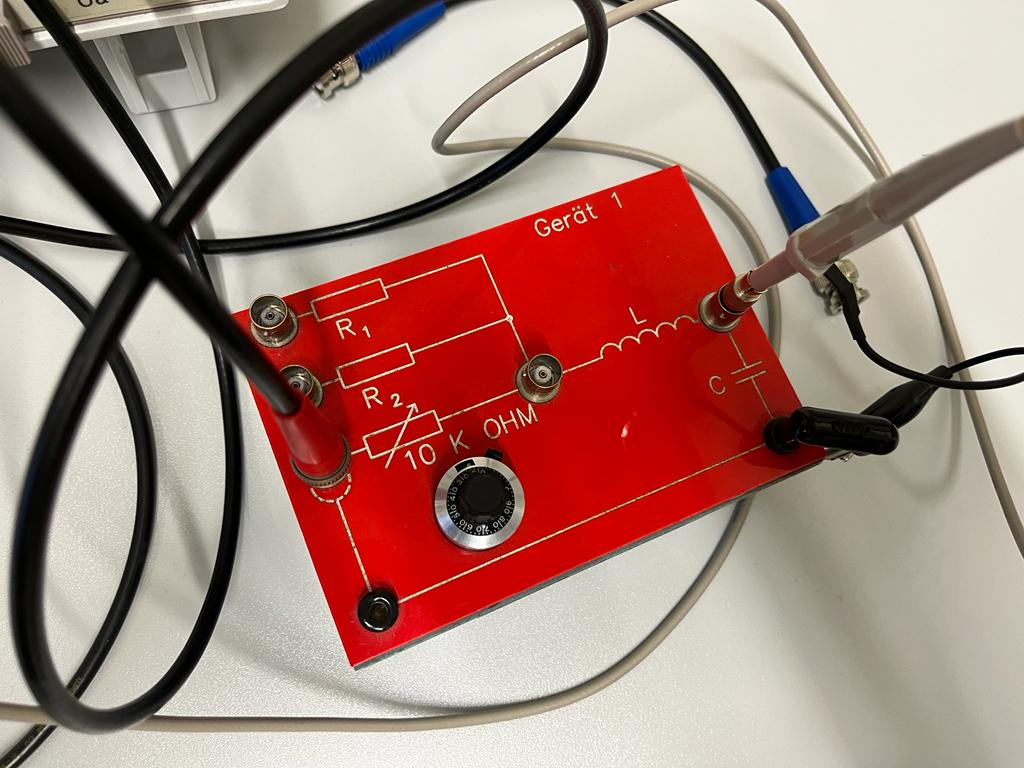
\includegraphics[width=80mm]{bilder/Ab4.jpeg}
    \caption{Ein Bild des Geräts 1 mit Tastkopf.\label{Abbildung4}}
\end{figure}

\begin{figure}[H]
    \centering
    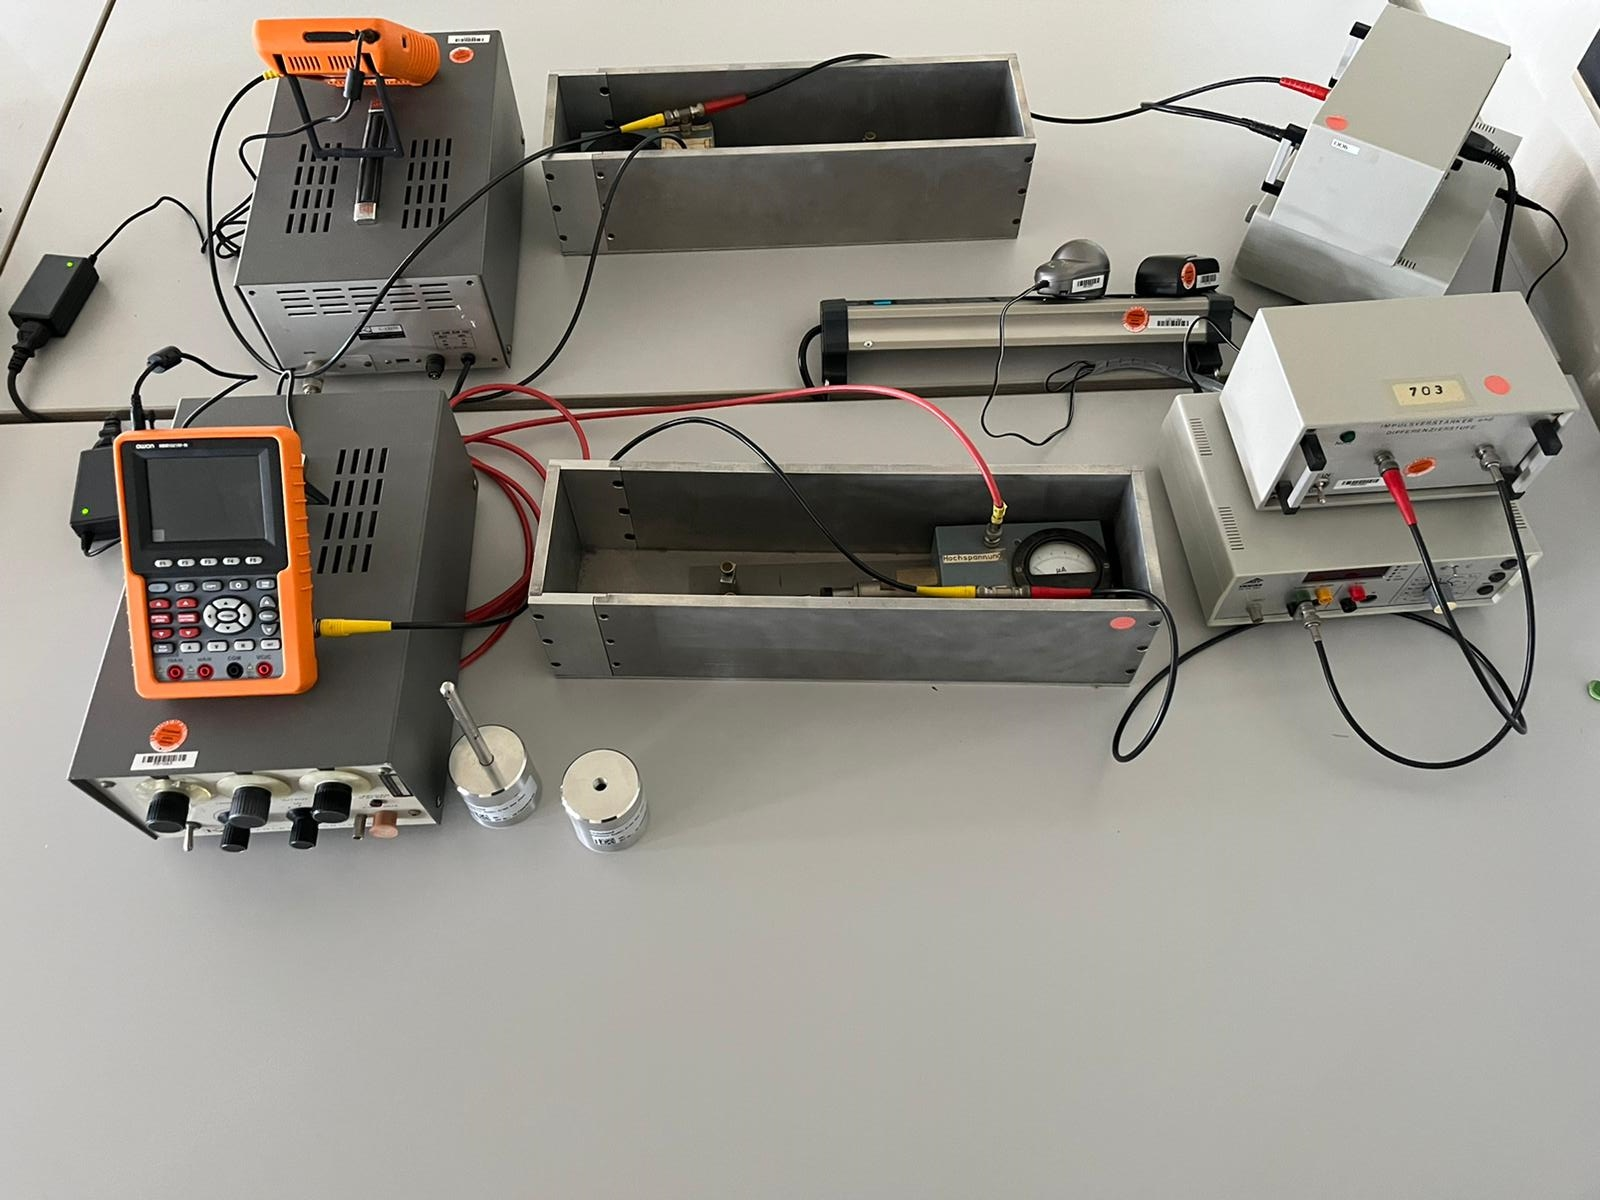
\includegraphics[width=90mm]{bilder/Ab5.jpeg}
    \caption{Übersicht auf den Kompletten Versuch (mit kleiner Erweiterung welche in Aufgabe 3 wichtig wird). \label{Abbildung5}}
\end{figure}
\section{Auswertung}

Die Werte für die Induktivität \textbf{I}, den Festwiderstand \textbf{R} und den Kondensator \textbf{C}
für das Gerät (Gerät 1) was in diesen Versuch verwendet wurde sind:


\begin{align*}
    \textbf{I} = (16,87 \pm 0,05)\,\unit{\milli\henry} \,\,\,\,
    \textbf{R} = (67,2 \pm 0,1)\,\unit{\ohm} \,\,\,\,
    \textbf{C} = (2,060 \pm 0,003)\,\unit{\nano\farad}.
\end{align*}

\begin{flushleft}
    Wichtig hierbei zusagen ist noch, dass die Festwiderstände, kleine Wertunterschiede vorweisen die aber nicht sehr groß sind und deshalb beide Widerstände den Wert \textbf{R} haben. \\
    Die gewählte Frequenz $\textbf{\text{f}} = 250\,\unit{\hertz} $ mit einem verstellbaren Widerstand bis zu $10\,\unit{\kilo\ohm}$.
    Der Widerstand ist festgelegt auf $\textbf{\text{R}} = 0,2\,\unit{\kilo\ohm} $.
\end{flushleft}

\begin{center}
    X-Achseneinstellung (Zeit): $10\,\unit{\micro\second} $ pro Einheit \\
    Y-Achseneinstellung (Spannung):  $ 0,2\,\unit{\volt} $ pro Einheit \\
\end{center}

\newpage

\begin{table}
    \centering
    \caption{Die Tabelle der Amplitude in Zeitabhängigkeit.}
    \label{Tabelle1}
    \begin{tabular} {c  c}
        \toprule
        {$U_\text{c}  \mathbin{/}  \unit{\volt}$} &
        {$t \mathbin{/}  \mu \unit{\second}$} \\
        \midrule
        0,80  \pm 0,1  & 0 \\
        -0,60 \pm 0,1  & 10,0 \pm 0,1  \\
        0,58  \pm 0,1  & 20,0 \pm 0,1  \\
        -0,44 \pm 0,1  & 29,5 \pm 0,5  \\ 
        0,43  \pm 0,01 & 38,5 \pm 0,5  \\
        -0,32 \pm 0,02 & 48,5 \pm 0,5  \\
        0,32  \pm 0,01 & 58,5 \pm 0,5  \\
        -0,22 \pm 0,01 & 67,9 \pm 0,01 \\
        0,24  \pm 0,01 & 77,0 \pm 0,05 \\
        -0,18 \pm 0,01 & 86,0 \pm 0,5  \\
        0,17  \pm 0,05 & 97,0 \pm 0,01 \\
        \bottomrule
    \end{tabular} 
\end{table}

\begin{figure}
    \centering
    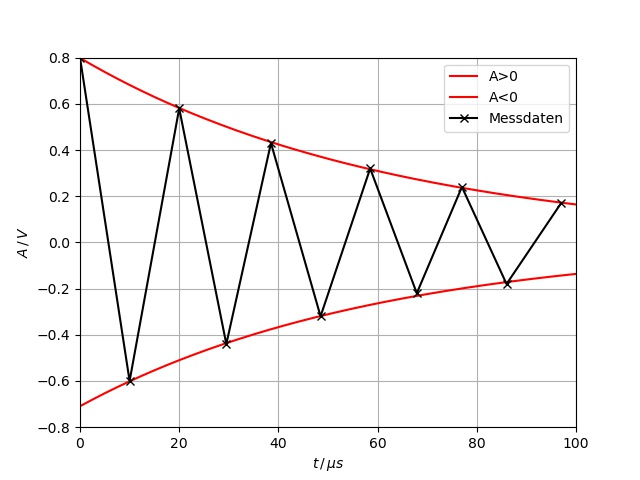
\includegraphics[width=90mm]{bilder/Ab10.jpeg}
    \caption{ Die Darstellung der Amplitude in Zeitabhängigkeit der Tabelle \ref{Tabelle1}. \label{Abbildung10} }
\end{figure}


\begin{align}
    \intertext{Die Einhüllende wird dargestellt in der Abbildung \ref{Abbildung10} mit den Werten aus der Tabelle \ref{Tabelle1} durch:}
    \text{A} = \text{A}_{0} \cdot e^{-2\,\pi\,\mu\,\text{t}}\,. \label{15}
    \intertext{Die Werte $\text{A}_{0}$ sowie $\mu$ lassen sich mit Hilfe einer Ausgleichsrechnung bestimmen:}
    \text{A}_{0} = (0,79 \pm 0,023)\,\unit{\ohm} \notag  \\
    \mu_{1}  = (0,0165 \pm 0,000940)\, \frac{1}{\unit{\second}} \notag
    \intertext{Der effektive Widerstand lässt sich durch umformen der oben genannte Funktion ausrechnen:}
    \text{R}_{\text{eff},1} = \mu_{1} \cdot 4\,\pi\,\cdot L = (0,00349 \pm 0,0016)\,\unit{\ohm}\,, \notag
    \intertext{ebenso die Abklingdauer}
    \text{T}_{\text{ex},1} = \frac{1}{2\,\pi\,\mu_{1}} = \frac{2\,\text{L}}{2\,\text{R}} = (9,645 \pm 0,321)\,\unit{\second} \notag
    \intertext{Vergleicht man nun die Werte des effektiven Widerstandes $\text{R}_{\text{eff},1}$ und den vorgegebenen Widerstand $\text{R} = (67,2 \pm 0,1)\,\unit{\ohm}$, so fällt auf, dass es eine Differenz von $-67,196\,\unit{\ohm}$ vorhanden ist.} \notag
\end{align}

\begin{align*}
    \intertext{Um den aperiodischen Widerstand im Grenzfall zu untersuchen, wurde der Graph so eingestellt, wie in Abbildung {\ref{Abbildung8}} zu sehen.
    Durch das Ablesen ergibt sich für $\text{R}_{\text{ap}}$ einen Wert von}
    \text{R}_{\text{ap}} = 2,2\,\unit{\kilo\ohm} = 2,2 \cdot 10^3\,\unit{\ohm}\,.
    \intertext{Der theoretische Wert lässt sich wie in der Formel (\ref{5}) bestimmen:}
    \text{R}_{\text{ap}} = \sqrt{\frac{4\,\text{L}}{\text{C}}} = (5723 \pm 0,013) \cdot 10^3\,\unit{\ohm}.
    \intertext{Die Abweichung beträgt 3,523 \unit{\kilo\ohm}, welches sich auf weitere Bauelemente zurückführen lassen kann, da wir nur $\text{R}_{1}$ bzw. $\text{R}_{2}$ gegeben haben, wurden andere Widerstände vernachlässigt.
    Somit haben wir es mit einem systematischen Fehler zu tun.
    Da $\text{R}_{\text{ap}}$ empirisch bestimmt wurde, können (größere) Messfehler auftreten.} 
\end{align*}


\begin{table}[H]
    \centering
    \caption{Frequenzabhängigkeit der Kondensatorspannung.}
    \label{Tabelle2}
    \begin{tabular} {c   c   c   c}
        \toprule
        {$ \text{U}_{0} \mathrm{/} \unit{\volt} $} &
        {$ \text{U}_{\text{C}} \mathrm{/} \unit{\volt} $} &
        {$ \frac{\text{U}_{\text{C}}}{\text{U}_{0}} $} &
        {$ \text{f} \mathrm{/} \unit{\kilo\hertz} $}\\
        \midrule
        4,8 & 0,52 & 0,1083 & 5  \\
        4,8 & 0,56 & 0,116  & 10 \\
        4,8 & 0,68 & 0,141  & 15 \\ 
        4,2 & 1,15 & 0,273  & 20 \\
        4,2 & 1,29 & 0,307  & 22 \\
        4,2 & 1,60 & 0,380  & 24 \\
        4,2 & 1,89 & 0,45   & 26 \\
        4,2 & 1,70 & 0,404  & 28 \\
        4,2 & 1,30 & 0,309  & 30 \\
        4,2 & 1,00 & 0,238  & 32 \\
        4,2 & 0,80 & 0,190  & 34 \\
        4,2 & 0,61 & 0,145  & 36 \\
        4,2 & 0,505& 0,120  & 38 \\
        4,2 & 0,50 & 0,119  & 40 \\
        \bottomrule
    \end{tabular} 
\end{table}


\begin{figure}[H]
    \centering
    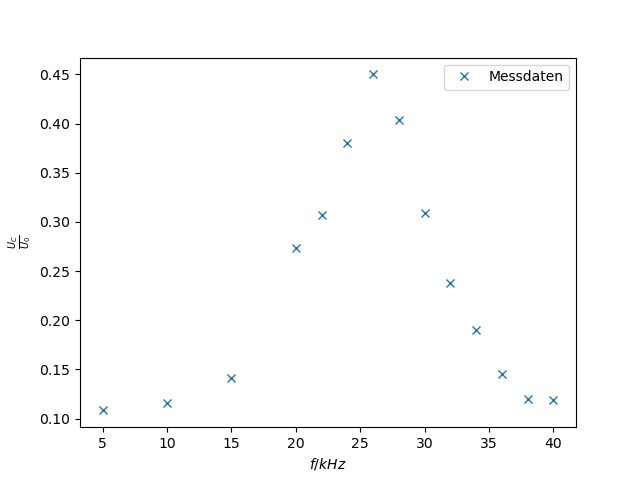
\includegraphics[width=90mm]{bilder/Ab11.jpeg}
    \caption{Darstellung der Werte $\frac{\text{U}_{\text{C}}}{\text{U}_{0}}$ in Frequenzabhängigkeit aus der Tabelle \ref{Tabelle2}. \label{Abbildung11} }
\end{figure}

\begin{align}
    \intertext{Die Güte q wurde experimentell bestimmt zu: $ \text{q}_{\text{e}} = 0,45 $.}
    \intertext{Man betrachte, dass unsere Spannung $ \text{U} = 2\,\unit{\volt}\mathbin{/}\text{Div} $, sowie $ \text{U}_{\text{C}} = 0.5\,\unit{\volt} \mathbin{/}\text{Div} $ bzw. $ 0.2\,\unit{\volt} \mathbin{/}\text{Div}  $
    am Oszilloskop eingestellt wurde. Der theoretische Wert lässt sich durch die Gleichung}
    \text{q} = \frac{1}{\omega_{0}\,\text{RC}} \quad mit \quad \omega_{0} = \sqrt{\frac{1}{\text{LC}}} \label{16}
    \intertext{ermitteln zu}
    \text{q} = 42,58 \pm 0,15 \quad mit \quad \text{R}_{2} = 67,2 \notag  \\
    Abweichung: \frac{\text{q}_{\text{exp}} - \text{q}_{\text{theo}}}{\text{q}_{\text{theo}}}\,. \notag \\
    \text{Die Abweichung hierbei beträgt}\,\, -98\%\,. \notag
    \intertext{Anschließend wird unsere Resonanzkurve mit einer linearen Gerade ergänzt. Die Gerade befindet sich bei}
    \frac{\text{U}_{\text{C}}}{\text{U}_{0}} = \frac{\text{q}_{\text{e}}}{\sqrt{2}} = 0,318\,. \notag
\end{align}

\begin{align*}
    \intertext{Zudem werden Halbwertsbreiten an den Punkten, welche sich mit dem Graphen kreuzen, aufgestellt.
    Der ermittelte Wert lautet}
    \nu_{+} - \nu_{-} = 7 \cdot 10^3\,\unit{\hertz} \\
    \intertext{Theoretisch: mit der Formel (\ref{14}):} 
    \nu_{+} - \nu_{-} = \frac{117\,\unit{\ohm}}{16,87\,\unit{\milli\henry}} = (6,9 \pm 0,000012) \cdot 10^{3}\,\unit{\hertz}  \notag\\
    \text{Die Abweichung hierbei beträgt}\,\, 1,15\%\,.
\end{align*}

\begin{align}
    \intertext{Die Phasenverschiebung der ersten drei gemessenen Werte beläuft sich bei einer Frequenz von $15\,\unit{\hertz}$ auf $10\,\unit{\micro\second}$. 
    Die Phasenverschiebung der restlichen gemessenen Werte beläuft sich bei einer Frequenz von $30\,\unit{\hertz}$ auf $6\,\unit{\micro\second}$.
    Eine ganze Phase beträgt $20\,\unit{\micro\second}$}
    \intertext{Die Berechnung einer Phase geht über die Formel}
    \left(\frac{\text{A}}{\text{B}} \right) \cdot 360°\,. \label{17}
    \intertext{Wobei \textbf{A} $D/V$ zwischen den Kästchen ist und \textbf{B} die komplette Phase ist.} \notag
\end{align}


\begin{figure}[H]
    \centering
    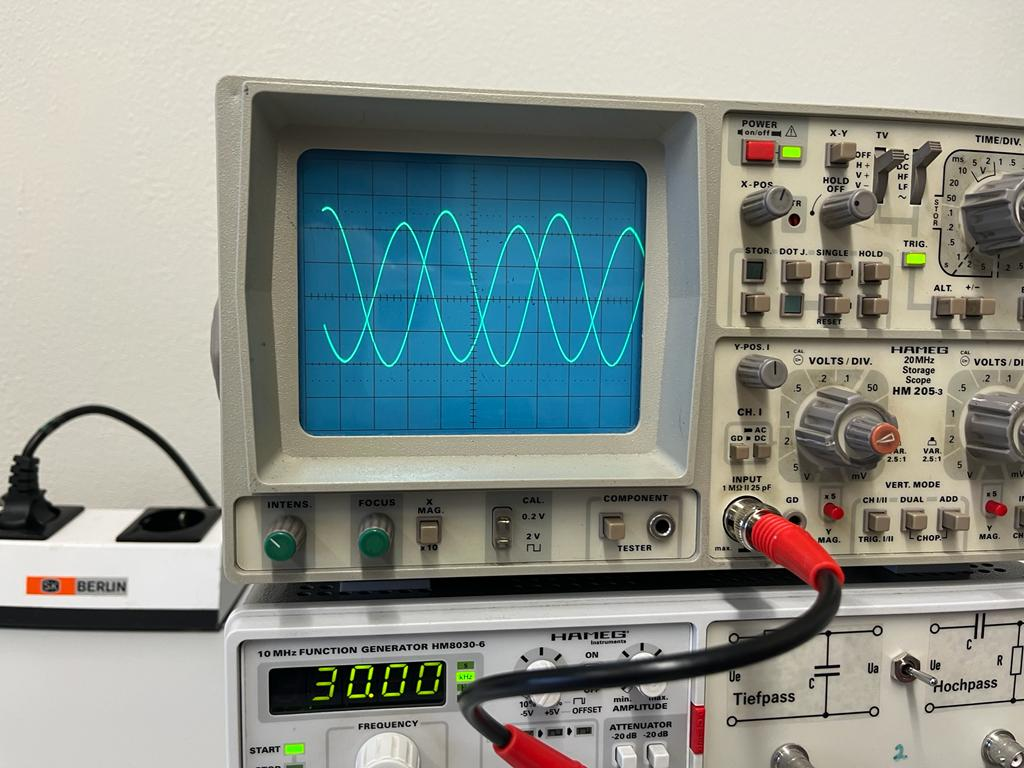
\includegraphics[width=76mm]{bilder/Ab12.jpeg}
    \caption{Die Phasenverschiebung am Oszilloskop verbildlicht.\label{Abbildung12}}
\end{figure}

\begin{table}[H]
    \centering
    \caption{Frequenzabhängigkeit der Kondensatorspannung.}
    \label{Tabelle3}
    \begin{tabular} {c  c  c}
        \toprule
        {$ \nu \mathbin{/} 10^{3}\,\unit{\hertz} $} &
        {$ \text{t} \mathbin{/} \mu \unit{\second}$}  &
        {$ \phi \mathbin{/} \unit{\degree} $}\\
        \midrule
        15 & 1 & 17,9  \\
        30 & 6 & 107   \\
    \end{tabular} 
\end{table}




\section{Diskussion}

\begin{flushleft}
    Betrachtet man die Auswertung, weichen drei Werte stark von dem theoretischen Wert ab. 
    Wie beim ersten Versuch dargestellt stellt sich ein Wert heraus, welcher eine große Abweichung vorweist.
    Das $\mu_{1}$ wurde mithilfe von der Einhüllenden $\text{A}= \text{A}_{0} \cdot e^{-2\pi\,\mu\,t}$ berechnet.
    Zwei mögliche Gründe dafür sind das falsches Ablesen der Werte, oder die falsche Berechnung mithilfe eines Darstellungsprogramms. 
    Jedoch scheinen die abgelesenen Werte realistisch, bezogen auf die Darstellung in dem Diagramm \ref{Abbildung10}.
    Die Dadurch folgende Differenz von $ 67,196\,\unit{\ohm} $ lassen sich durch das nicht betrachten der Innenwiderstände des Oszilloskops, welche ungefähr bei $50\, \unit{\ohm}$ \cite{rohde} liegen, erläutern.
    Die Güte ist ebenfalls ein Faktor, welcher Abweichungen des theoretischen Werts vorweist. Die Breite der Resonanzkurve befindet sich im Toleranzbereich. 
    Bei genauer Betrachtung weichen viele Werte ab, dies lässt sich auf überwiegend systematische Fehler zurückweisen.
\end{flushleft}
\section{Anhang}

\begin{flushleft}
    \begin{figure}
        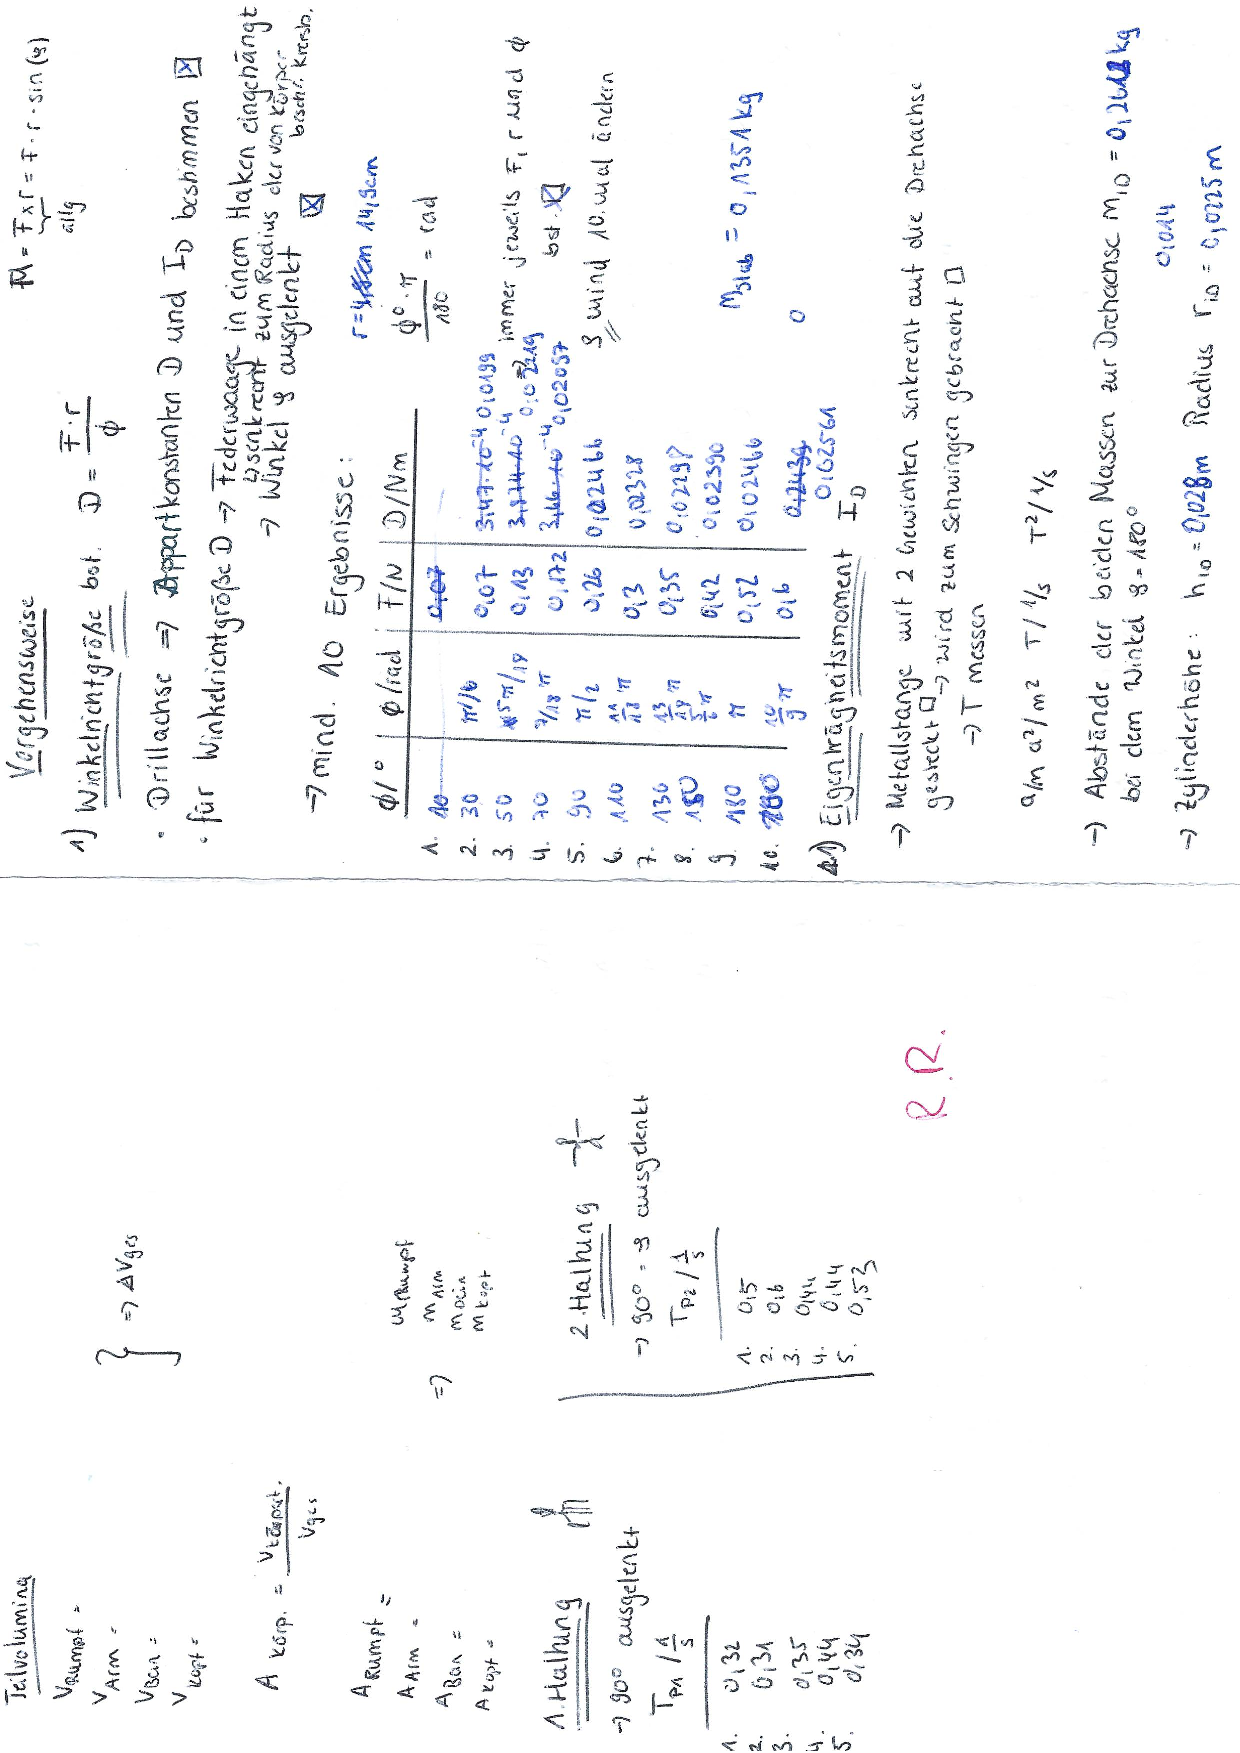
\includegraphics[width = 17cm]{Messdaten/Messdatenanhang1.pdf}
    \end{figure}
    \begin{figure}
        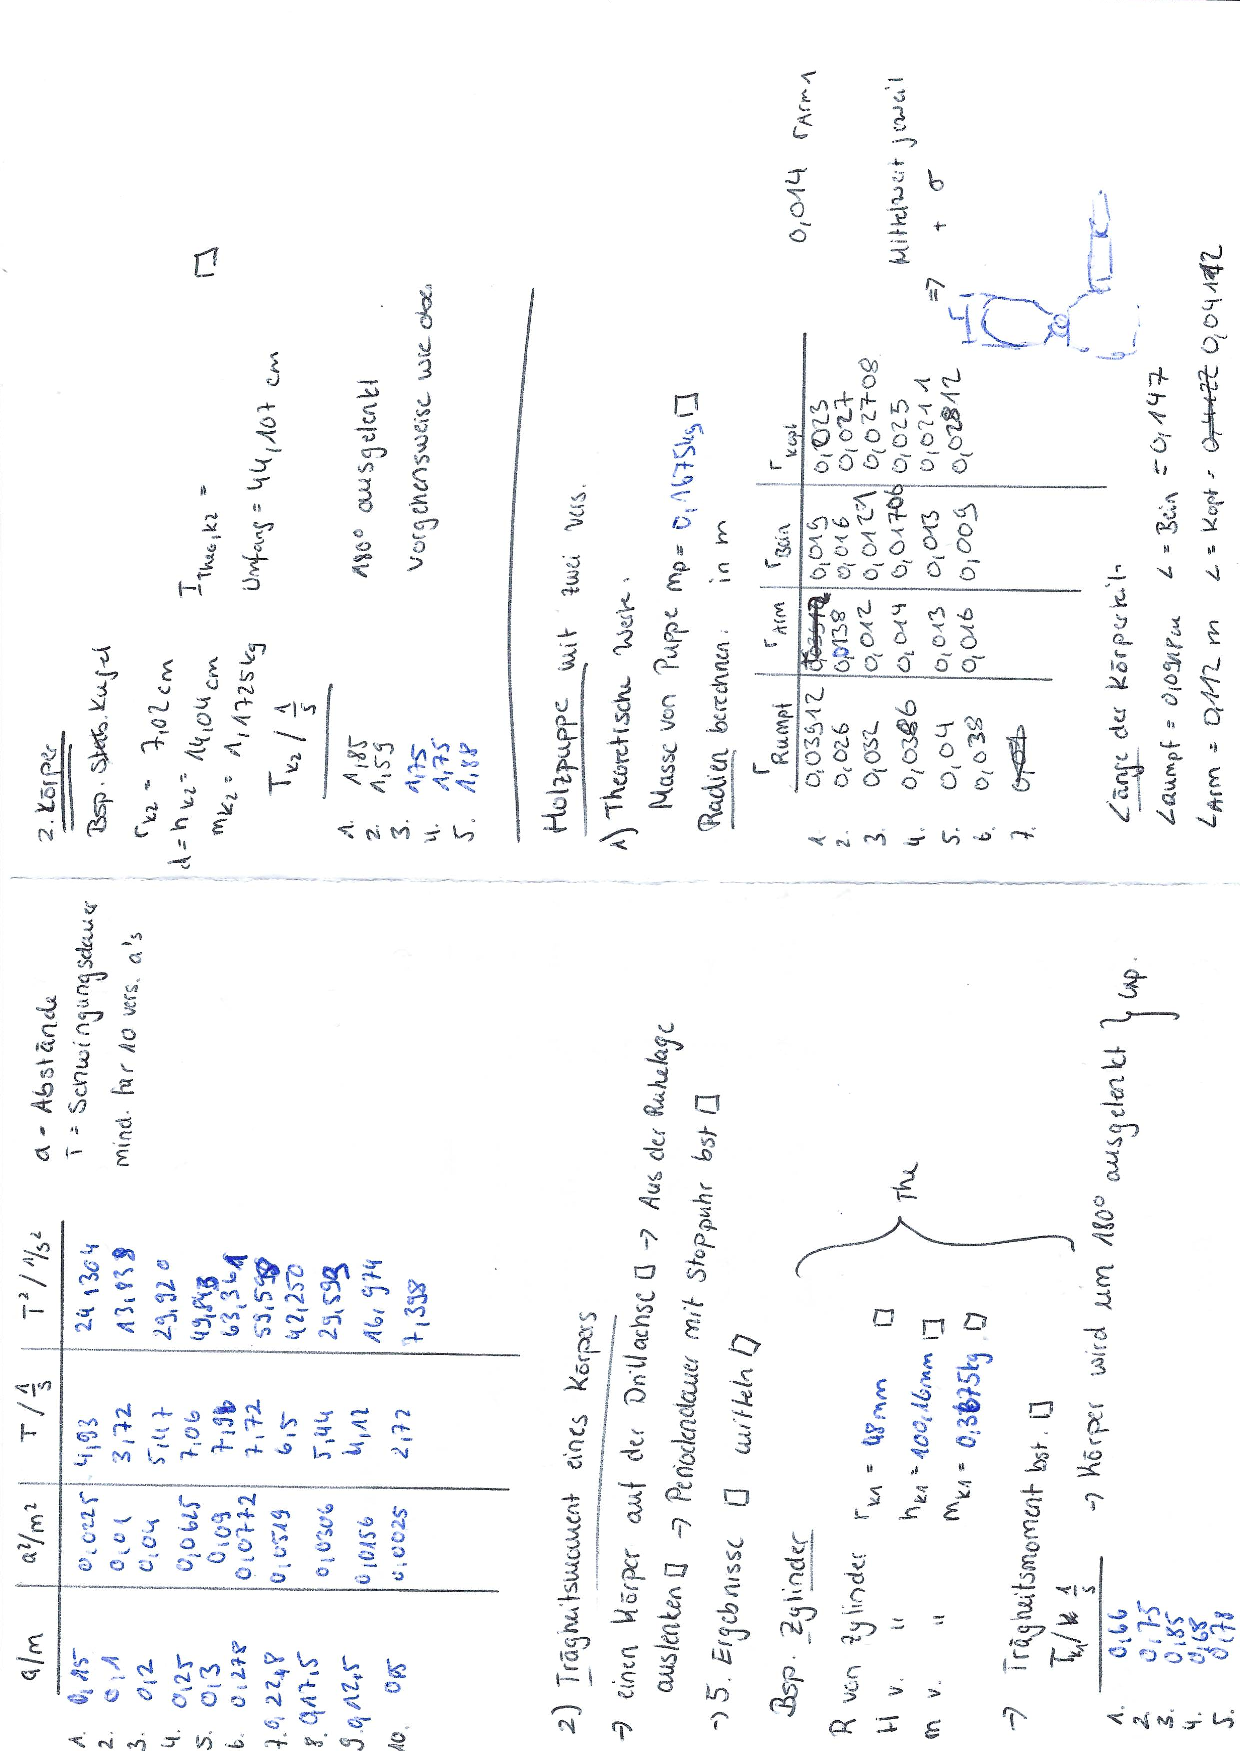
\includegraphics[width = 17cm ]{Messdaten/Messdatenanhang2.pdf}
    \end{figure}
\end{flushleft}

\nocite{*}
\printbibliography{}

\end{document}